\documentclass{article}
\author{Isaac B Goss\\ James Hahn\\ Jonathan Dyer}
\title{Assignment 21}
\date{25 Oct 2017}

\usepackage{amsmath}
\usepackage{amsthm}
\usepackage{enumitem}
\usepackage[margin=0.8in]{geometry}
\usepackage{graphicx}

% ============ USED FOR OUR FORMAT ============
\newtheorem{thm}{Claim}
\providecommand{\prob}[1]{\section*{Problem #1}}
\providecommand{\soln}{\textbf{Solution: }}
\providecommand{\image}[1]{
    \begin{center}
        \includegraphics[width=0.3\textwidth]
            {#1}
    \end{center}
}
\providecommand{\tightlist}{
    \setlength{\itemsep}{0pt}\setlength{\parskip}{0pt}
}
\providecommand{\reducible}[2]{
  \textbf{#1} $\leq$ \textbf{#2}
}

% ============ USED FOR CODE LISTINGS ============
\usepackage{listings}
\usepackage[usenames,dvipsnames,svgnames]{xcolor}
\definecolor{javagreen}{rgb}{0.25,0.5,0.35}
\lstset{
    basicstyle   = \footnotesize,
    commentstyle = \color{javagreen},
    frame        = single,
    language     = C,
    stringstyle  = \color{orange},
    numbers      = left,
    showstringspaces=false,
    deletekeywords = {len, max, format, min},
    morekeywords = {yield, function, then, do, to},
    keywordstyle = \color{blue},
    escapeinside = {(*}{*)},
    mathescape
}


\begin{document}
\maketitle

\prob{13}
\begin{enumerate}[label=(\alph*)]
 \item This is NP-hard. We will show \reducible{Clique}{$\dfrac{3}{4}$IndependentSet}.
       \begin{lstlisting}
function Clique(Graph G, int k)
    //want $\dfrac{3}{4}n$ to be at least k, since all k-cliques contain (k-1)-cliques, etc.
    while k $> \dfrac{3}{4}n$
        add some leaf vertex anywhere in G
    return 34Clique(G, k)
 \end{lstlisting}

 \item This is NP-hard. We will show \reducible{$\dfrac{3}{4}$Clique}{$\dfrac{3}{4}$IndependentSet}. This is identical to the \reducible{Clique}{IndependentSet} that we did previously.
       \begin{lstlisting}
function 34Clique(Graph G, int k)
    return 34IndependentSet(G$^C$, k)
  \end{lstlisting}

 \item This is NP-hard. We will show \reducible{Clique}{CliqueAndInd}
       \begin{lstlisting}
function Clique(Graph G, int k)
    let H = new independent set of k vertices
    if CliqueAndInd(G+H,k)  // if the known independent set plus G passes the AND test,
        return 1            // then G$\ni$(k-clique)
  \end{lstlisting}

 \item This is NP-hard. We will show  \reducible{Clique}{CliqueOrInd}\\
       We simply need to eliminate any independent set in G without compromising a possible clique.
       The easiest way to do this is to simply add a new vertex and connect it to all vertices in G.
       Then any clique will just be one vertex larger, which is of course fine since (k+1)-cliques of course contain k-cliques.
       \begin{lstlisting}
function Clique(Graph G, int k)
    let H = G $\times$ v    // cross product of G and one vertex
    return CliqueOrInd(H, k)
       \end{lstlisting}

 \item This is NP-hard. We can show \reducible{$\dfrac{3}{4}$Clique}{$\dfrac{3}{4}$CliqueAndInd} in a way analogous to the above proof.

 \item This is $\rule[0.5ex]{4em}{0.1ex}\hspace{-4em}\text{NP-hard}$ too hard. I'm done.
\end{enumerate}

\pagebreak
\prob{14}
Each clause of a CNF Boolean formula can be viewed as a linear inequality in a system thereof,
in the sense that \textbf{all} inequalities must be satisfied,
just as \textbf{all} clauses in a CNF forumla must be.
Let's represent every variable in the CNF by a variable of the same name in our system.
Then, each vaiable can either be added to or subtracted from the inequality based on whether it is inverted in the respective CNF clause.

We want these variables to only be assigned 1 or -1 (representing logic true and false, respectively), so we need to add an extra condition for each variable.
Some options are that for each variable $x$, we could choose one of the following:
\begin{itemize}
  \item $-1 \leq x \leq 1$, but this still allows for assignment of intermediate values.
  \item $n^2 = 1$, but this is not a linear equation.
  \item $(-1)^x$ could be used as the variable to satisfy, but this of course is not linear either.
  \item $|x| = 1$ is the closest to linear, so this is what we'll use.
\end{itemize}

Each inequality then is satisfied when any of the terms evaluate to positive 1.
To accomplish this, we can put negative the number of terms in the equation.

Let's look at an example to explain this.
Consider the following CNF forumla.

\begin{align*}
    (\overline{x} \lor y \lor z) \land (x \lor \overline{y} \lor z \lor w \lor \overline{u})
\end{align*}

This can be transformed into the following system of linear inequalities.

\begin{align*}
    -x + y + z &\geq 2\\
    x - y + z + w -u &\geq 4\\
    |x| = |y| = |z| = |w| = |u| &= 1
\end{align*}

Thus, this here is our ultimate reduction.

\begin{lstlisting}
function CNF-Decider(F)
    S = a system of linear inequalities
    for clause C in F do
        I = a new linear inequality, default "0 $\geq$ 0"
        for literal l in C do
            subtract 1 from right-hand-side of I
            let v = the variable in literal l
            if v has not been seen in S then
                add equality "|v| = 1" to S // make sure only 1 or -1 is assigned.
            if l = $\overline{v}$ then
                add term "-v" to left-hand-side of I
            else
                add term "+v" to left-hand-side of I
        add inequality I to S
    return LinearIneqDecider(S)
\end{lstlisting}

\pagebreak
\prob{19}

We set up $G$ as stated in the hint.
The we add an edge between all vertices in $R$ which represent the edges of $H$, and the vertices incident to them.
Further, we make all vertices in $G - R$ adjacent to the single source vertex $s$.
As an example, this leaves us with $G$ looking something like this:

\begin{center}
    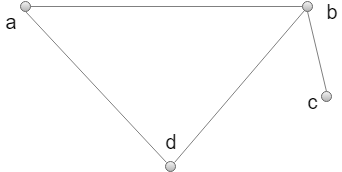
\includegraphics[width=0.3\textwidth]{a21p19first}
    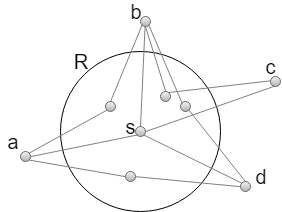
\includegraphics[width=0.3\textwidth]{a21p19graph}
\end{center}

Where the original graph $H$ is on the left, and our construction $G$ is on the right. Note, for the sake of brevity, I will call a solution to the problem presented here a \textbf{walk}.

Note that we can find a vertex cover of size 2 in $H$, $\{b, d\}$.
Likewise, $U = \{b, d\} \cup R$ is a walk of $G$.
But, we cannot create any vertex cover of size 1, no matter what vertex we choose.
In the same way, no single vertex can be added to $R$ to create a walk.
Keep this example in mind when considering the following algorithm and following proof of correctness.

\begin{lstlisting}
function VertexCover(H, l)
    let R = $\{ e \text{ (as a vertex)} \ |\ e \in E(H) \}$ $\cup$ $\{s\}$
    let T = V(H)
    let G = (V = T $\cup$ R, E = $\emptyset$)
    for vertex v in T do
        add edge between s and v in G
    for vertex e in R do
        let uv = e // the vertices to which e is adjacent in H
        add edge between e and v in G
        add edge between e and u in G
    return ThisProblem(G, R, |R| + l)
\end{lstlisting}

\begin{proof}
    In order for this algorithm to correctly solve vertex cover, we must have that some vertex cover $S$ exists for $H$ if and only if $R \cup S$ is a walk for $G$.
    \begin{itemize}
        \item $S$ is a vertex cover $\implies$ $R \cup S$ is a walk.

        Assume this is not so.
        Then there exists some vertex $e \in R$ which has no path to some other vertex in $R$.
        One of these vertices must be completely disconnected in $G$; we shall say it is $e$ without loss of generality
        [if both were adjacent to any vertex outside of $R$, then they would be connected through $s$].
        We know that $e$ has exactly 2 neighbors $u,v \in V(G)$.
        Thus, $u, v \not\in U \implies u, v \not\in S$.
        Thus, we have a contradiction.
        Some edge is not covered in our vertex cover.

        \item $R \cup S$ is a walk $\implies$ $S$ is a vertex cover.

        Again, assume this is not the case.
        Then there exists some edge $e = uv$ which is not covered.
        That is, $u, v \not\in S \implies u, v \not\in R \cup S = U$.
        Then, $\exists e \in R$ which has no neighbors in $U$.
        This is a contradiction of our walk.
    \end{itemize}
\end{proof}

\end{document}
